%%%%%%%%%%%%%%%%%%%%%%%%%%%%%%%%%%%%%%%%%
% Masters/Doctoral Thesis 
% LaTeX Template
% Version 1.43 (17/5/14)
%
% This template has been downloaded from:
% http://www.LaTeXTemplates.com

% Original authors:
% Steven Gunn 
% http://users.ecs.soton.ac.uk/srg/softwaretools/document/templates/
% and
% Sunil Patel
% http://www.sunilpatel.co.uk/thesis-template/
%
% License:
% CC BY-NC-SA 3.0 (http://creativecommons.org/licenses/by-nc-sa/3.0/)
%
% Note:
% Make sure to edit document variables in the Thesis.cls file
%
%
% Modified and Adapted by Michael Lees 2020
%%%%%%%%%%%%%%%%%%%%%%%%%%%%%%%%%%%%%%%%%

%----------------------------------------------------------------------------------------
%    PACKAGES AND OTHER DOCUMENT CONFIGURATIONS
%----------------------------------------------------------------------------------------

\documentclass[11pt, oneside, dvipsnames]{Thesis} % The default font size and one-sided printing (no margin offsets)
\graphicspath{{Figures}} % Specifies the directory where pictures are stored


\usepackage[square, numbers, comma, sort&compress]{natbib} % Use the natbib reference package - read up on this to edit the reference style; if you want text (e.g. Smith et al., 2012) for the in-text references (instead of numbers), remove 'numbers' 
\usepackage[ruled,vlined]{algorithm2e}
\usepackage{amsmath}
% \usepackage{subfig}
\usepackage{subcaption}
\usepackage{enumitem}
\setlist{nolistsep}
\usepackage{booktabs}
\usepackage{algorithm2e}
\usepackage{custom_commands}

\usepackage{titlesec}
\DeclareMathOperator*{\argmin}{arg\,min}
\DeclareMathOperator*{\argmax}{arg\,max}
\title{\ttitle} % Defines the thesis title - don't touch this

\begin{document}
\section{DeGroot Model} \label{degroot_results} \subsection{PBS Scores} We
first proceed with analyzing the performance of the DeGroot model on
substantive agreement. \Cref{fig:pbs} shows the PBS of both the
deliberation and control group, and the simulation results for both instances.
As mentioned in \Cref{sub:americainonroom}, the PBS (PBS) is the
average of the 26 most polarizing questions, where a low PBS corresponds to
more liberal answers, and high PBS indicates more conservative answers. As
expected the model performs poorly at predicting the control group, as there
was no significant change for control group members. Similar to the control
group, the starting  PBS of the participants is a strong indicator for
their  PBS. Therefore the model at t=0 is already reasonably aligned with
the final  PBS. We see that after the first time step the PBS scores get
predicted more accurately, after which the model starts making larger
prediction errors. This is because the model keeps averaging all opinions until
a steady state is reaches in which most voters hold non-extreme positions.
Whether this is positive depends on reality, as
\citet{elsterMARKETFORUMThree2002} remarked, if deliberation is able to reach
full consensus, the model might give a glimpse into how this works. If this is
not the case however, then the model is overly naive suggesting that people
come to hold a weighted average of all original opinions. The latter seems more
likely.


\begin{figure}
	\begin{center}
		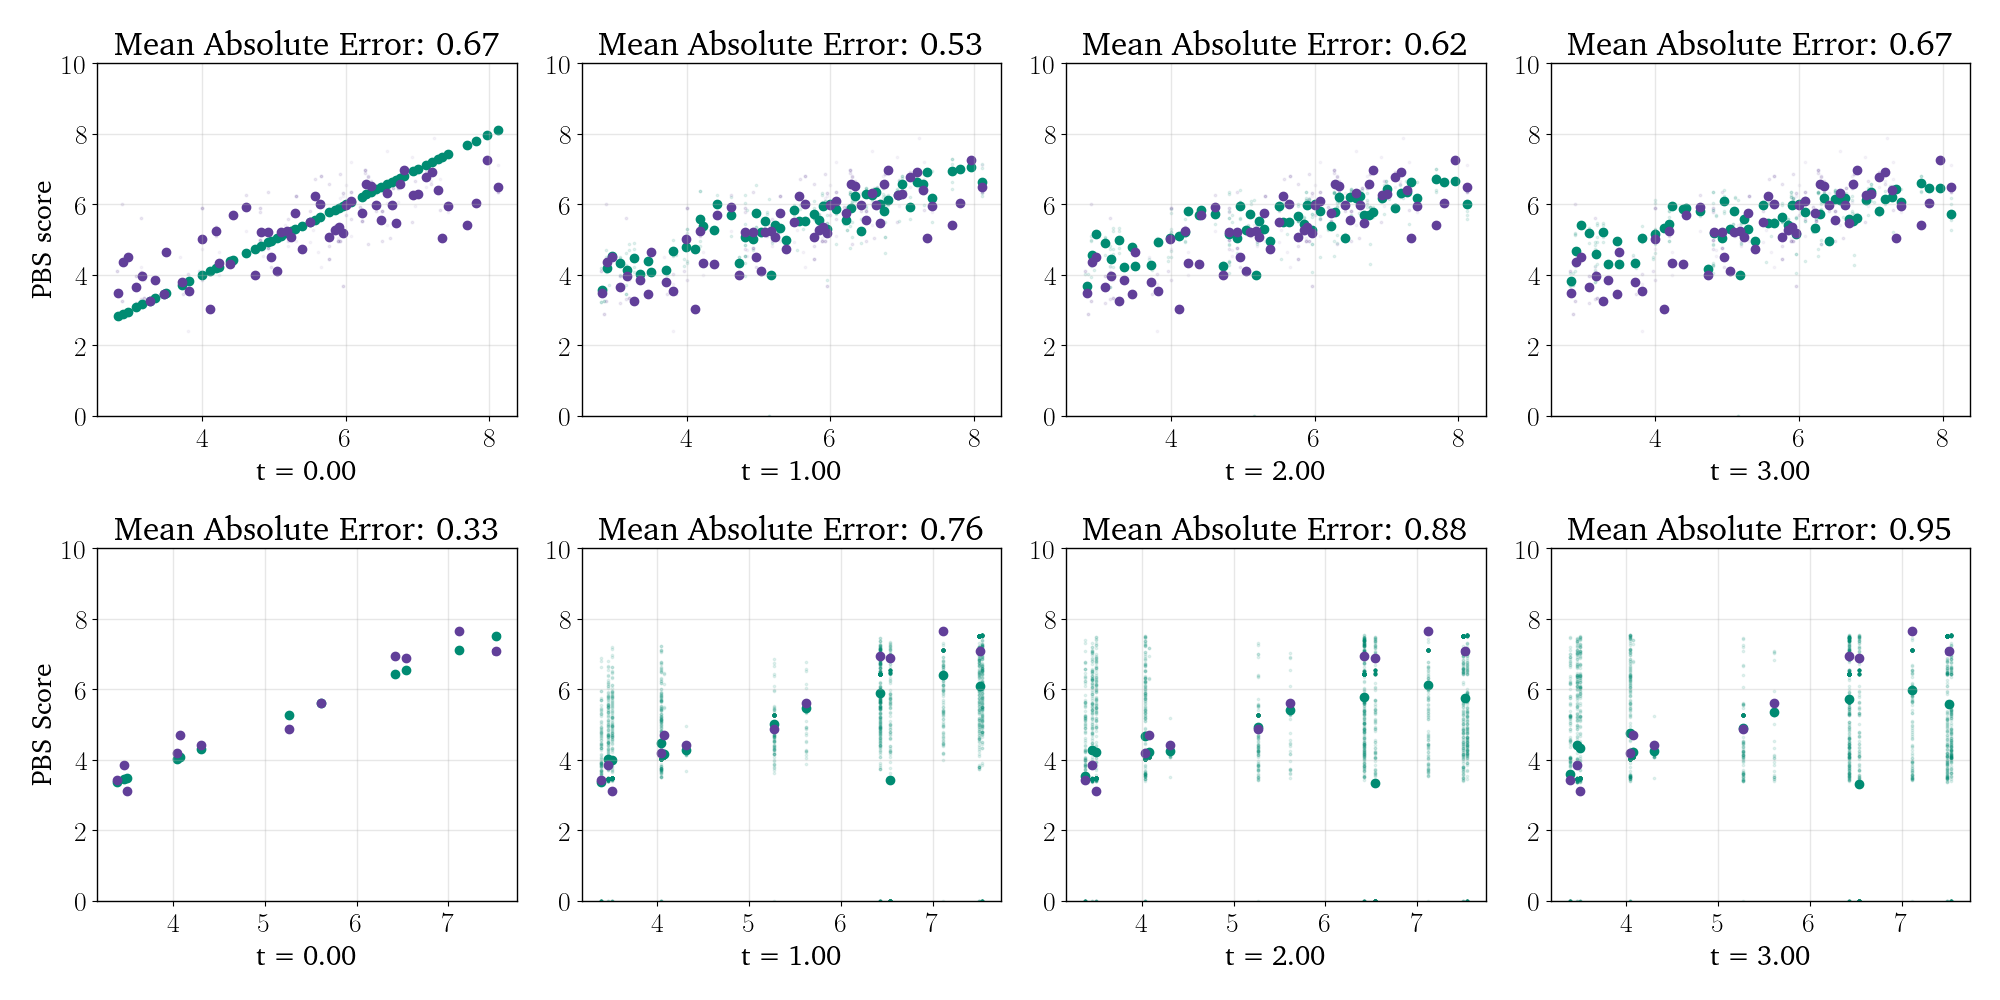
\includegraphics[width=0.95\textwidth]{Figures/pbs_scores.png}
	\end{center}
	\caption{ PBS, purple indicating the PBS score after deliberation in the original data, green indicates the results of the simulation in that time step.}\label{fig:pbs}
\end{figure}

\Cref{fig:delta_pbs} shows the change in  PBS for the deliberation group,
the original data shows most change happens in people with high  PBS,
getting lower PBS and thus becoming less extreme. The model does not capture
this effect, showing the most change for people with low initial  PBS in
later time steps. This might be because there is a correlation between PBS
score and knowledge. As shown by \citet{fishkinCanDeliberationHave2024}, most
extreme voters, in terms of PBS, seemed to also be the most knowledgeable, if
this was skewed towards voters with high PBS, then these voters would have more
effect on people's opinions in this model when using knowledge-based trust.
Looking at the binned errors in \Cref{fig:binned_errors}, we see that the model
performs better when we do not include knowledge, further indicating that
knowledge is a poor predictor of trust, or persuasiveness. Of course this claim
might be weakened by noting that knowledge in this case is measured by
questions regarding the current state of the America government, such as know
which party currently has a majority in the senate. Thus, this specific
knowledge might be insufficient to predict someone's persuasiveness on the
topic of immigration for example.


\begin{figure}
	\begin{center}
		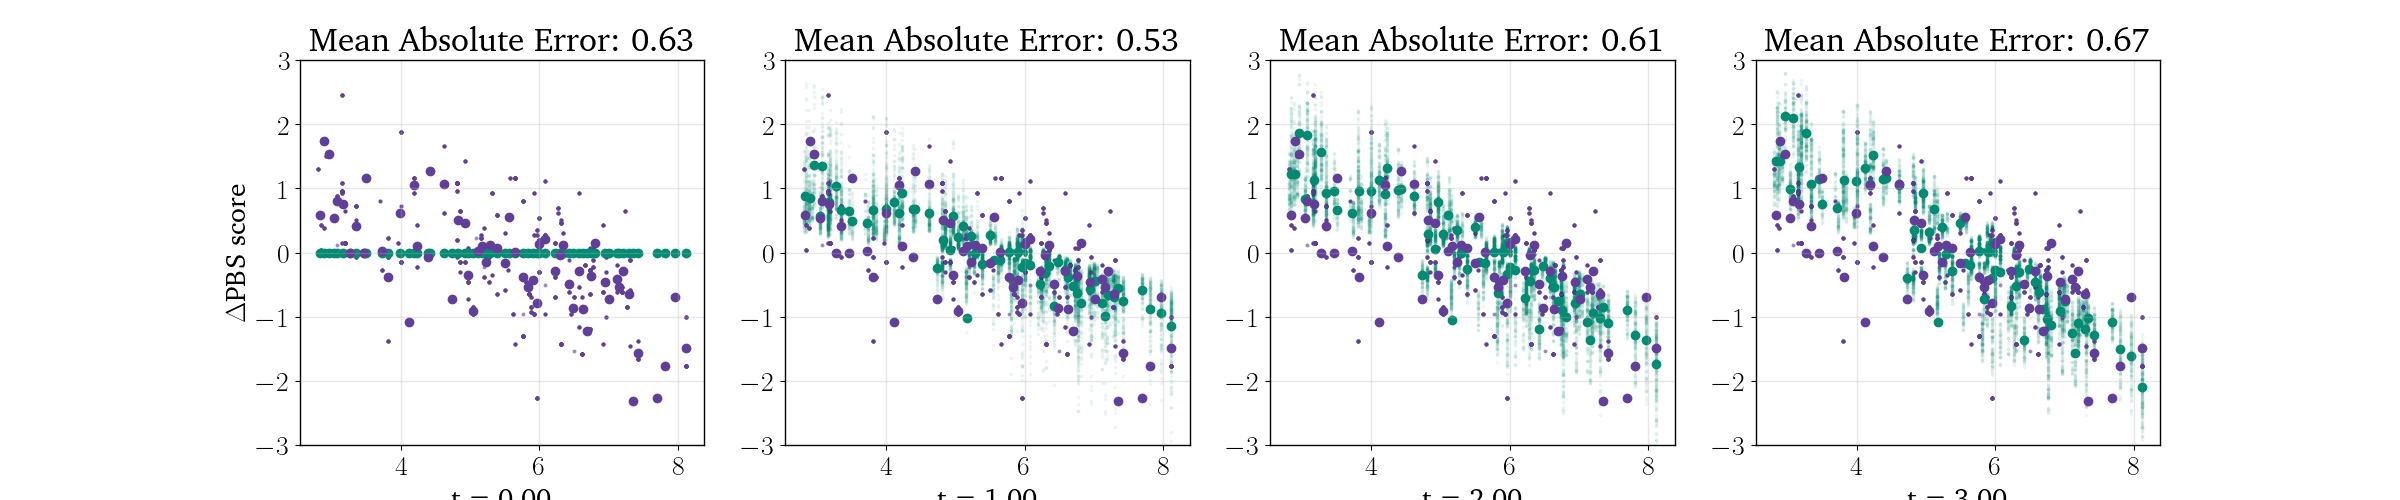
\includegraphics[width=\textwidth]{Figures/change_pbs_scores.png}
	\end{center}
	\caption{Change in  PBS, relative to the original, pre deliberation, measurement. The control is  omitted as there was no significant change.}\label{fig:delta_pbs}
\end{figure}


We note that this slight positive results appear only when the voters are
grouped by their original PBS, thereby giving the model reasonable predictive
power over a population of voters. We note that this hold even for different
sizes of bins. \Cref{fig:binned_errors} shows the progression of errors over
time when the error is calculated on a per-individual basis, and we find the
model consistently does worse than predicting someone to not change their
opinion, which is what t=0 indicates.

\begin{figure}
	\begin{center}
		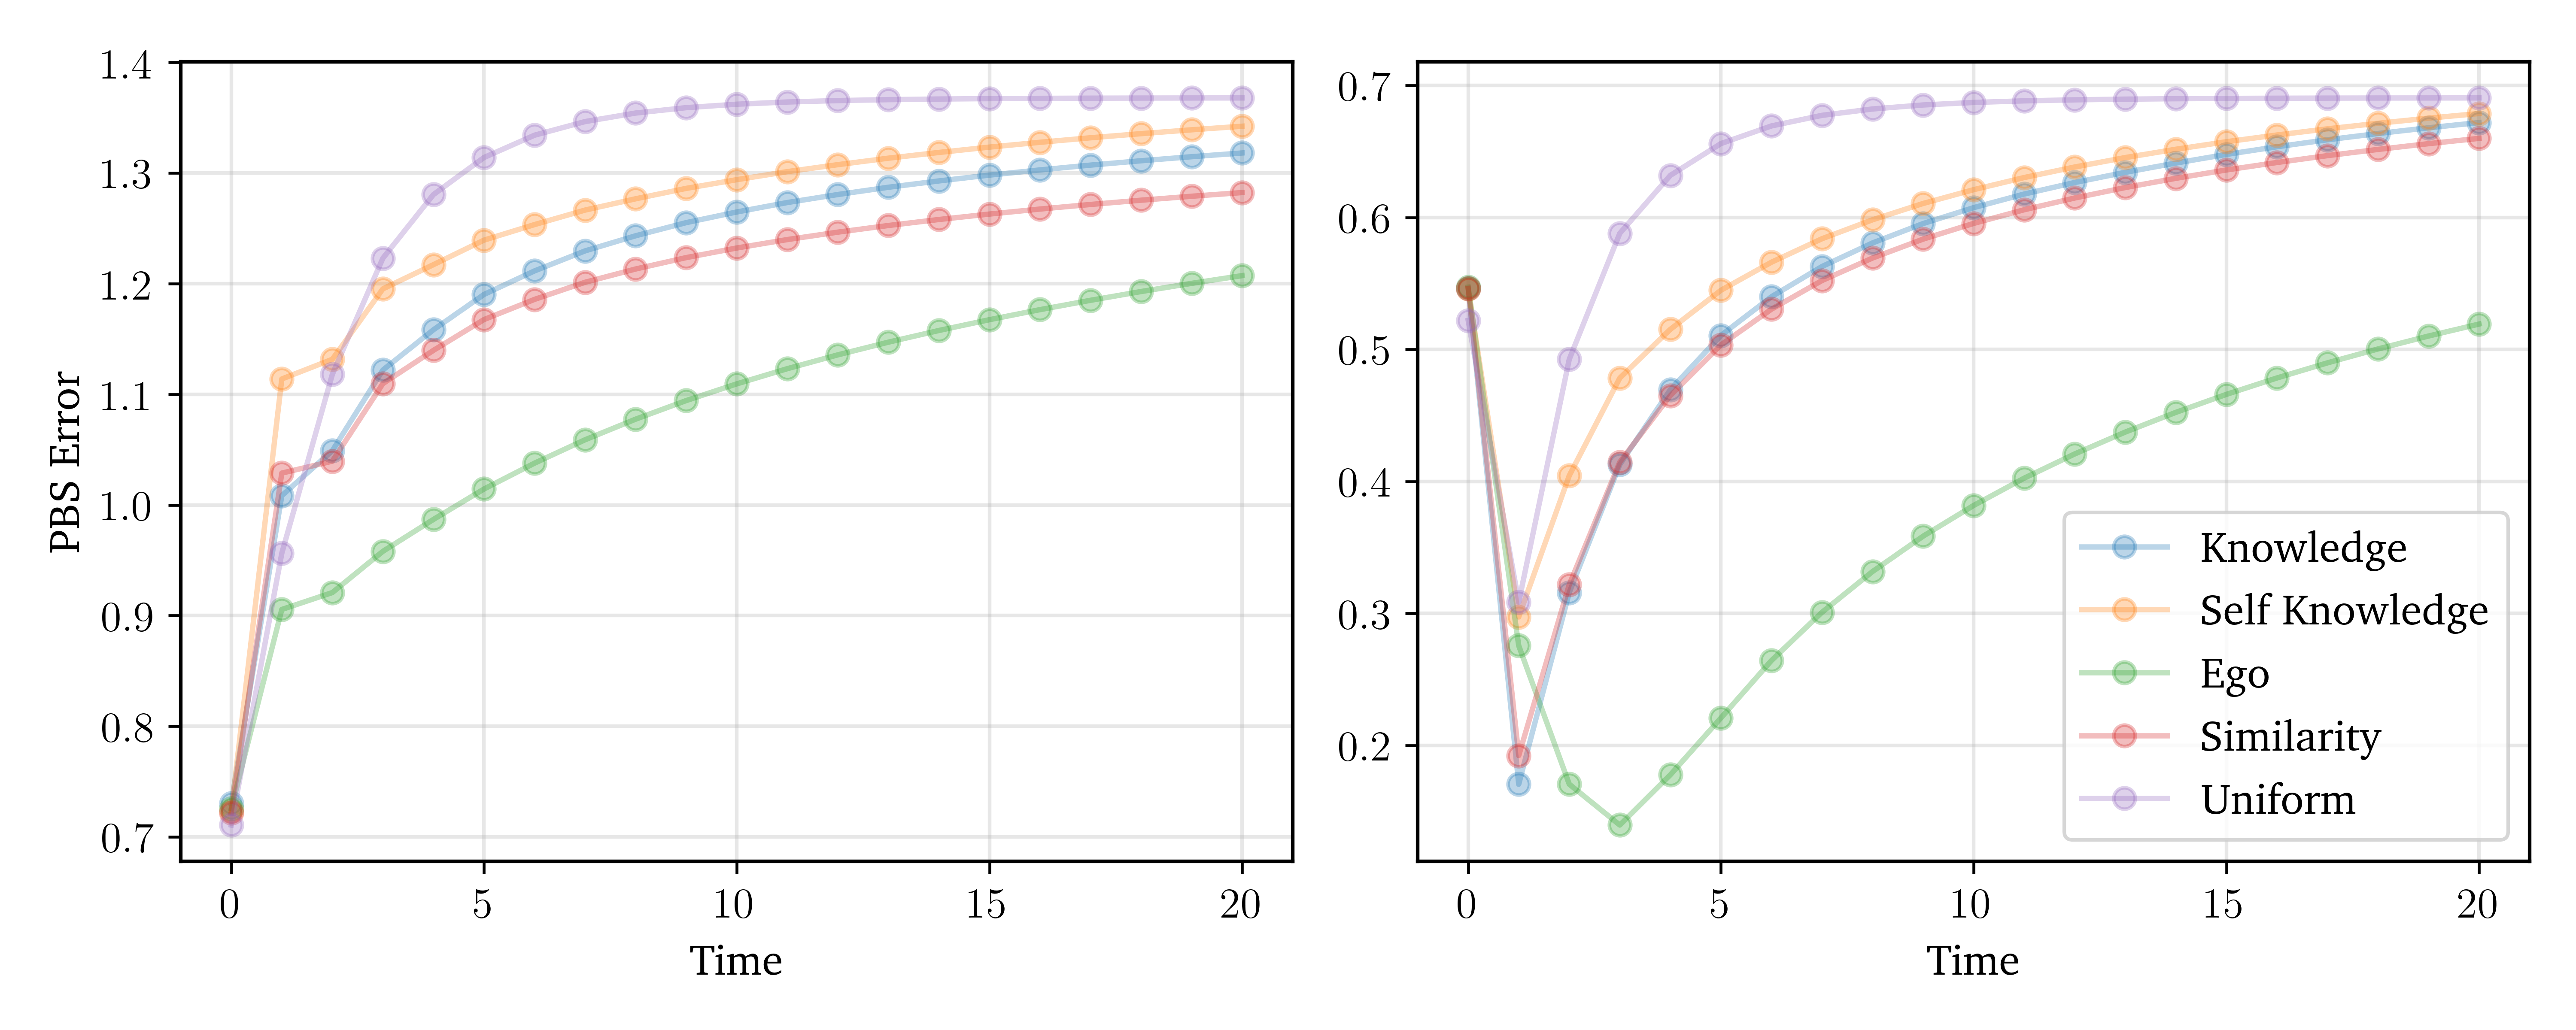
\includegraphics[width=0.95\textwidth]{Figures/errors_binned.png}
	\end{center}
	\caption{Prediction error of the model as a function of time, binned relative to the original  PBS.}\label{fig:binned_errors}
\end{figure}


\begin{figure}
	\centering

	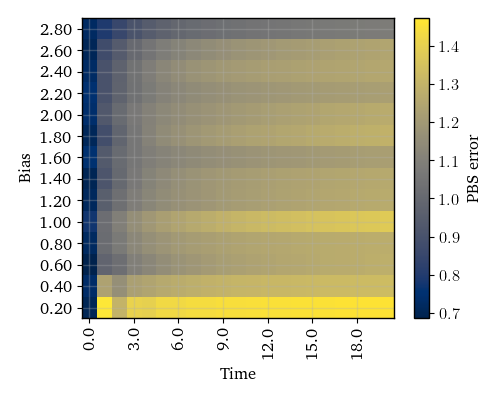
\includegraphics[width=0.6\textwidth]{Figures/bias_time_imshow.png}
	\hspace{1em}
	\caption{PBS Errors as a function of bias and time. bias acts as a damper, when bias is higher the model take longer to over estimate the change in opinion.}
	\label{fig:bias_slowdown}
\end{figure}

\Cref{fig:bias_slowdown} shows the relation between the bias factor and the PB
score, showing that the bias does not improve the models predictive power. As
one might expect a bias is ``slowing down'' the model. Because of this the
model is slower to diverge away from the true opinions.

% Here it is clear that generally the model performs best when both the number of
% candidates and the number of voters are low. We also not that though the error
% of the different candidate generators are comparable, they in general the
% Sample methods seems to results in larger errors, meaning that the model is
% less well able to capture circumstances where the alternative's opinions are
% not represented in the deliberating population. Finally, we see that The
% distribution of best biases skews to values around 1.3, thus indicating that
% even while deliberating, people tend to hold their opinion to be \textit{more}
% important than that of all other voters.
%
% We investigate this discrepancy between the two candidates generation methods
% now, to this end we look at the difference in error for all tested
% configuration.

% Now we T test on everything the Sample and Voter method

\subsection{Convergence}

From \Cref{theory}, we have seen that in the limit some matrices are
convergent, while some are not, in particular if the matrix is aperiodic, this
it is convergent. As we model the deliberation group as having fully connected
matrices, the matrices are aperiodic, and thus convergent. We look at the
distance between the estimated support matrix, and the true support matrix, to
get a sense of the rate of convergence. The distance in the element wise
$\ell_1$ norm.

\begin{figure}
	\begin{center}
		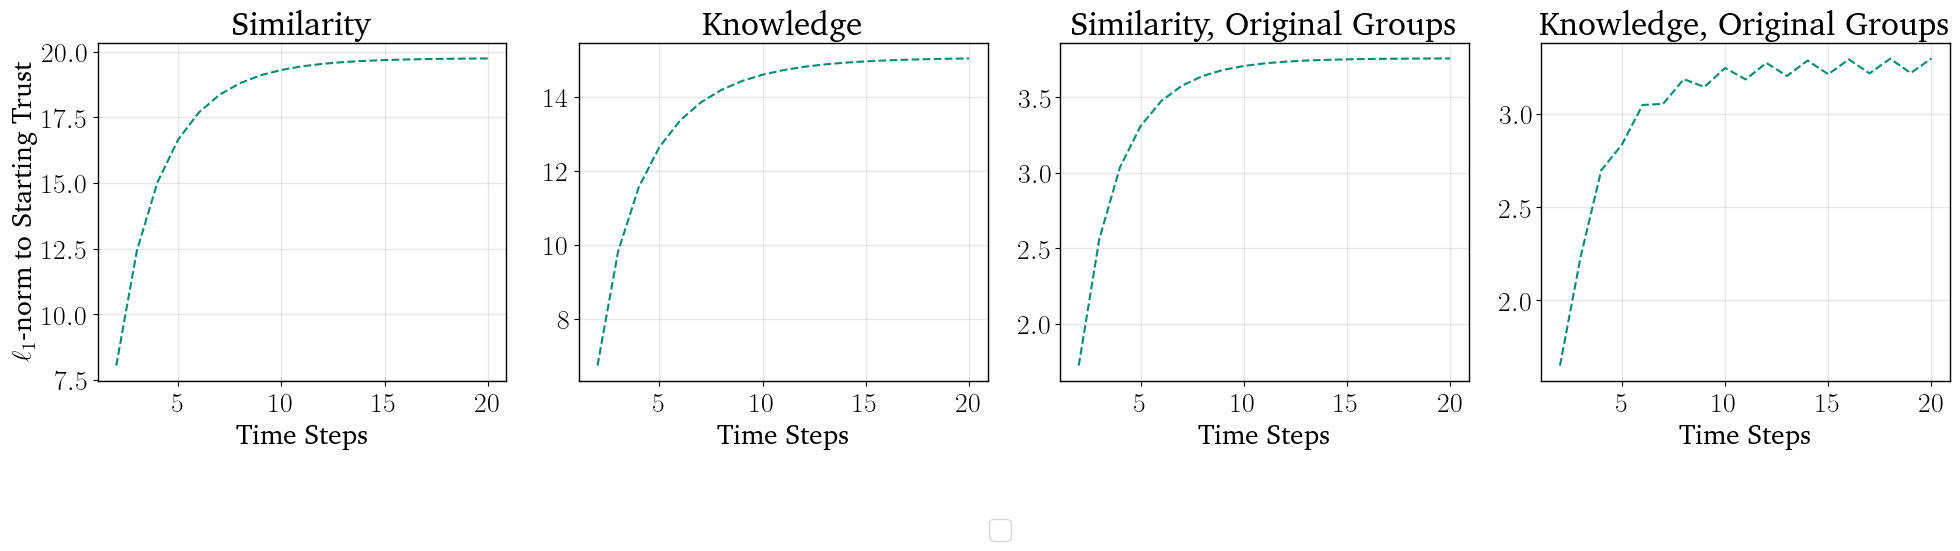
\includegraphics[width=0.95\textwidth]{Figures/convergence_groups.png}
	\end{center}
	\caption{Convergence of trust matrices, as measured by the $\ell_1$-norm between the trust matrix at the start and  trust matrix at the current time step
		t}\label{fig:convergence_big}
\end{figure}



% We now proceed to look at distance to single-peaked profiles, look at both
% voter removal and candidate removal. We show that for optimal bias, as
% deliberation progresses we see an increase in the proximity to single
% peakedness.
\section{Elections}

\begin{figure}[htbp]
	\centering
	\begin{minipage}{0.45\textwidth}
		\centering
		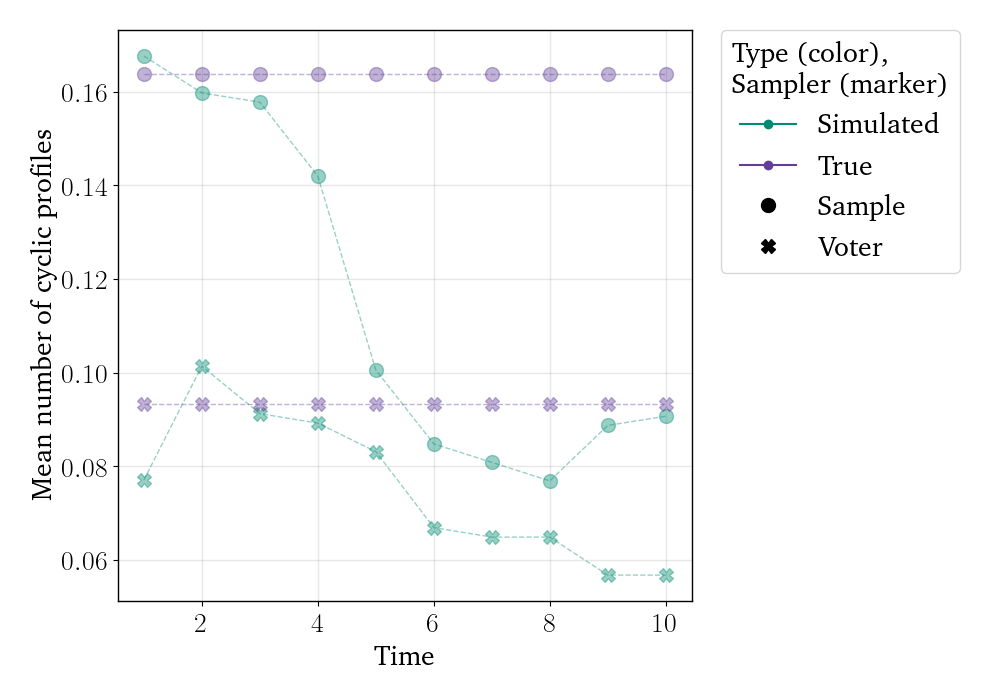
\includegraphics[width=\textwidth]{Figures/delib_Mean Number of Cyclic Profiles.png}
		\caption{The proportion of cyclic profiles remaining, 0 indicating that no cyclic profiles were present after deliberation.}
		\label{fig:degroot_cyclic}
	\end{minipage}\hfill
	\begin{minipage}{0.45\textwidth}
		\centering
		\vspace{-9pt}
		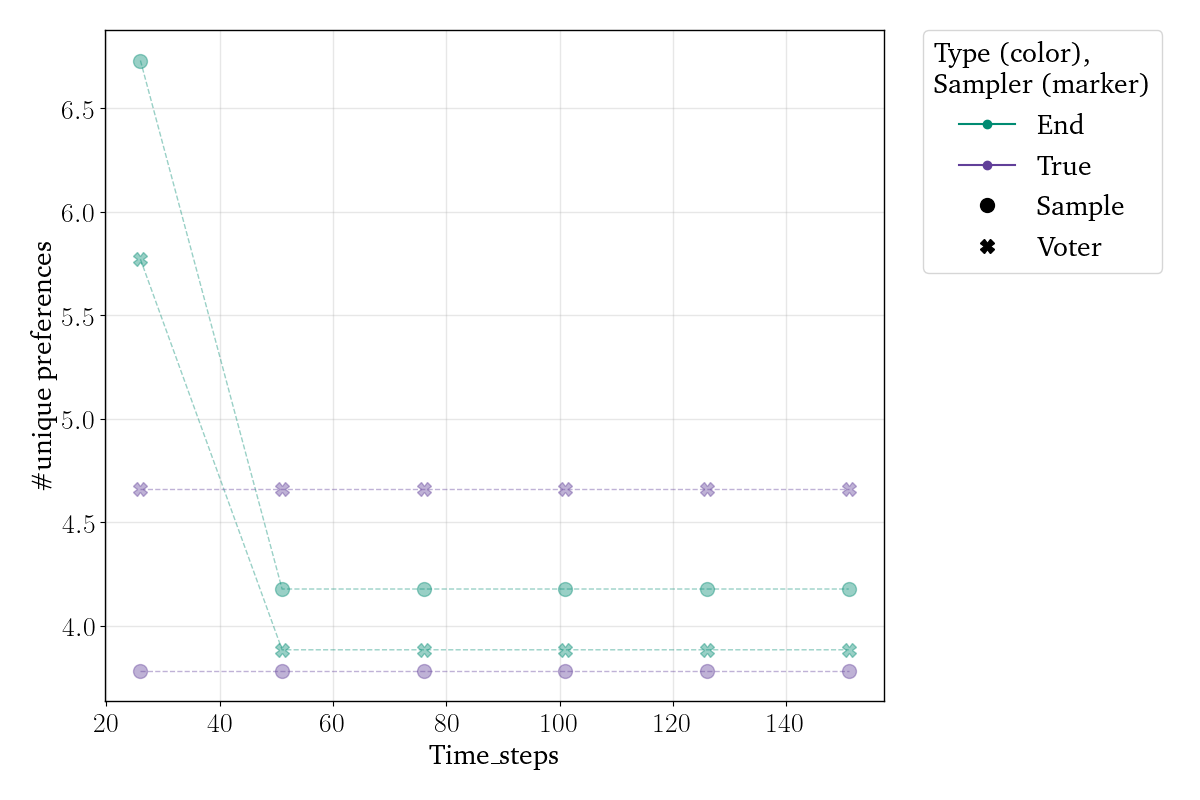
\includegraphics[width=\textwidth]{Figures/delib_number_Unique Preferences.png}
		\caption{Number of unique preferences at the final step of deliberation.}
		\label{fig:degroot_count}
	\end{minipage}

	\vspace{1em}

	\begin{minipage}{0.45\textwidth}
		\centering
		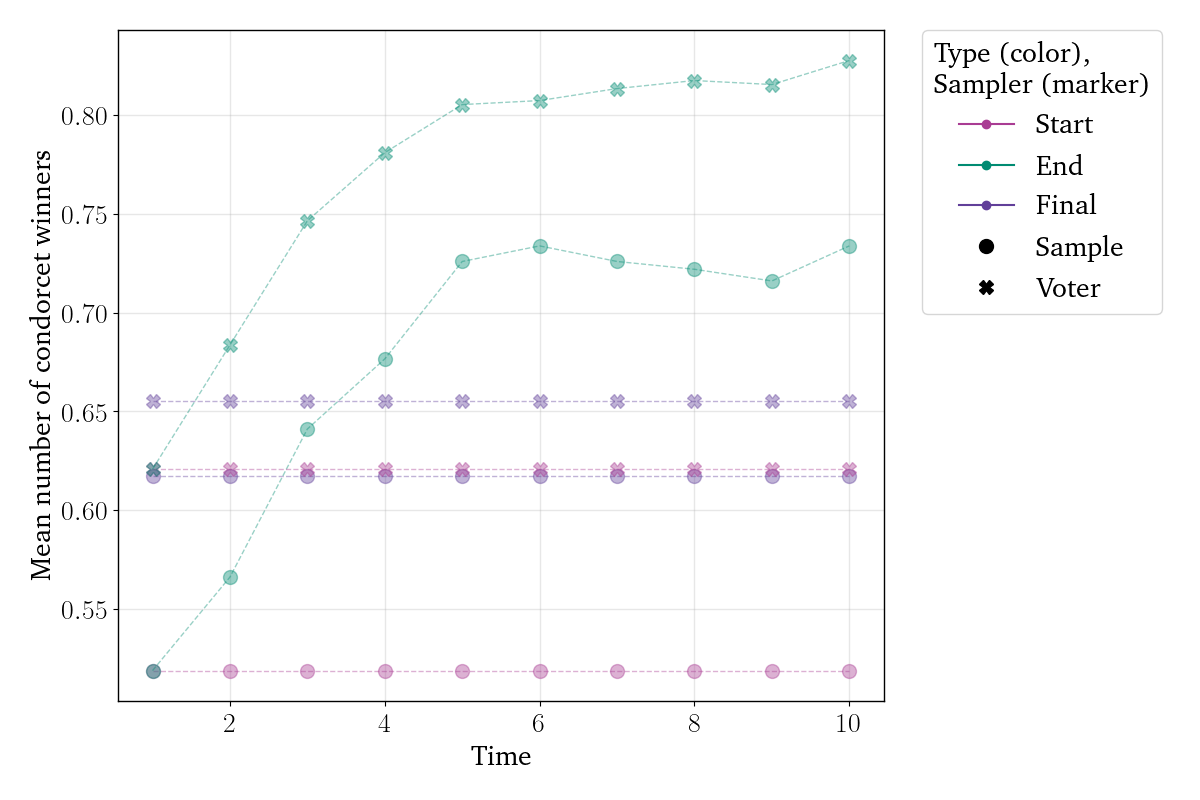
\includegraphics[width=\textwidth]{Figures/delib_Mean number of Condorcet winners.png}
		\caption{The proportion of Condorcet winners left after deliberation, value above one indicate Condorcet winners emerging during deliberation}
		\label{fig:degroot_condorcet}
	\end{minipage}\hfill
	\begin{minipage}{0.45\textwidth}
		\centering
		\vspace{-9pt}
		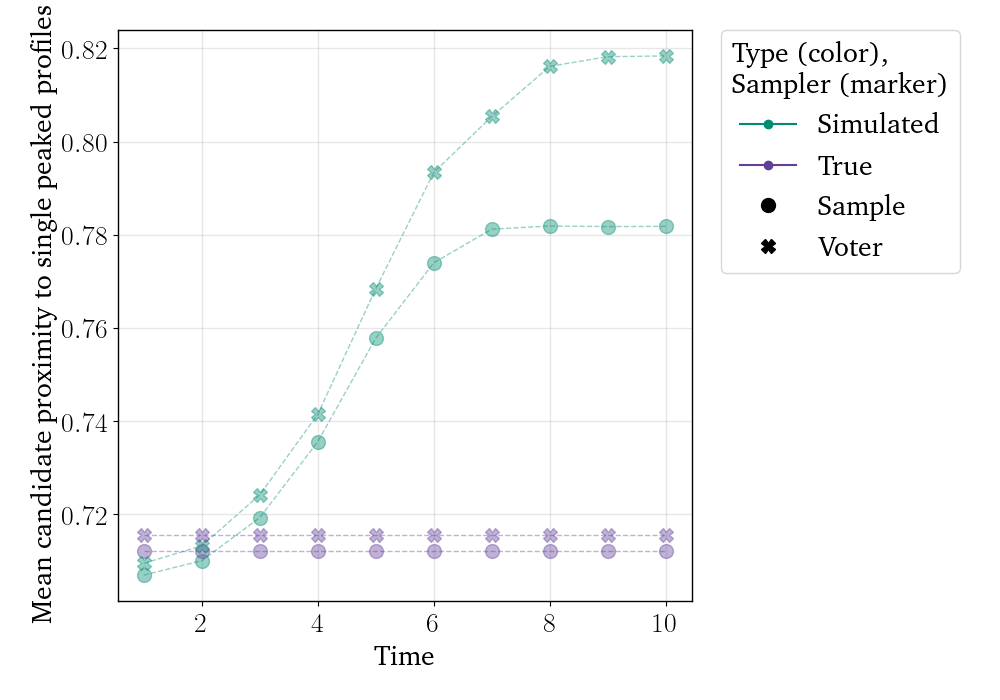
\includegraphics[width=\textwidth]{Figures/delib_Mean candidate proximity to single peaked Profiles.png}
		\caption{Proximity to single-peakedness after deliberation. Proximity to single-peakedness as defined in \Cref{section:related_work}.}
		\label{fig:degroot_single_peaked}
	\end{minipage}
\end{figure}


Firstly, looking at the different voter generation mechanisms, we find that in
general they do not affect the metrics much. The metric for which this is not
true is that of the fraction of elections with a Condorcet winner. Though
slightly unintuitive, we suspect the reason why a single voter's opinion is
more likely to result in a Condorcet winner than the average of 10 voters is
that the true opinions before deliberation were more polarized. As a result,
having multiple ``average'' candidates results in little difference between
them, while an individual voter is more likely to fall close to a large camp of
voters, and thus become a Condorcet winner through being closer to a majority
of voters.

Looking at the metrics evaluated on the model, we see similar results as with
the analysis for substantive agreement. At first the simulation starts far from
the metrics from the true score, then it moves towards it and overshoots it
until it starts to converge. Interestingly, for these metrics, the model does require more steps to converge to the same values as the true data.

\textcolor{gray}{This last analysis is very short and needs work}
\end{document}
